\documentclass[conference]{IEEEtran}
\IEEEoverridecommandlockouts
% The preceding line is only needed to identify funding in the first footnote. If that is unneeded, please comment it out.
\usepackage{cite}
\usepackage{amsmath,amssymb,amsfonts}
\usepackage{algorithmic}
\usepackage{graphicx}
\usepackage{textcomp}
\usepackage{xcolor}
\usepackage{natbib}


\def\BibTeX{{\rm B\kern-.05em{\sc i\kern-.025em b}\kern-.08e
    T\kern-.1667em\lower.7ex\hbox{E}\kern-.125emX}}
\begin{document}

\title{Blockchain y tablas hash}

\author{
    \IEEEauthorblockN{ Wilson Bryan Aguilar Siquigua}
    \IEEEauthorblockA{\textit{Machine Learning} \\
        \textit{Universidad Politécnica Salesiana}\\
        Quito, Ecuador \\
        waguilars@est.ups.edu.ec}
}

\maketitle

\begin{abstract}
    El blockchain es la forma de guardar la información de manera distribuida alrededor de miles de computadoras en el mundo, con el fin de que si existe alguna modificación de esta, las demás computadoras deben verificar si el cambio es verídico. De esta manera se asegura que no haya alteraciones de estos datos y evitar así el fraude. En este documento habalaremos acerca de como se logra esto, las aplicaciones que tiene esta tecnología y la relación que tiene con las tablas hash para que sean tan seguras.
\end{abstract}

\begin{IEEEkeywords}
    blockchain, bitcoin, transacción, hash
\end{IEEEkeywords}

\section{Funcionamiento}

Antiguamente las instituciones utilizaban libros donde registraban los movimientos y transacciones, el titular de este libro puede interactuar con otros interesados en consultar la información de este convirtiendose asi en una unidad central o intermediario. Esto viene a ser una red centralizada donde el titular de este libro tiene el control de todo el sistema y interviene en cada una de las transacciones que se pueden llevar a cabo.

\begin{figure}[htbp]
    \centering
    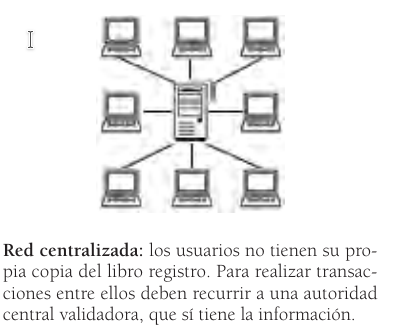
\includegraphics[scale=.8]{assets/images/red-centralizada.png}
    \caption{Red centralizada}
\end{figure}

El blockchain viene a cambiar todo esto, a través de un tipo de protocolo de código abierto, permitiendo que las bases de datos de esta sea de manera distribuida, eliminando asi a ``el intermediario o unidad central".

La tecnología blockchain es una tecnología que permite crear redes de libros de registros de transacciones electronicas o tambien bases de datos de transacciones, donde estos libros o bases de datos estan distribuidos entre los que son participantes de esta red. \cite{blockchain1}

Dentro de estas redes, cada uno de los usuarios o participantes actua como nodo y cada uno de ellos tiene una copia original de estos registros, por lo que cada usuario es libre de realizar transacciones directamente sin necesidad de un intermediario.

\begin{figure}[htbp]
    \centering
    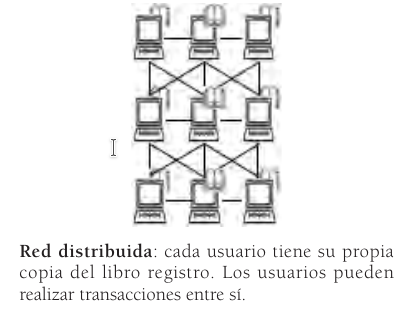
\includegraphics[scale=.8]{assets/images/red-distribuida.png}
    \caption{Red distribuida}
\end{figure}

El hecho de que cada usuario lleve el registro de las transacciones que se llevan a cabo, significa que estas deben ser validadas por cada uno de los nodos o participantes de esta red en base a su propia copia del registro, en caso de que un solo nodo no llegue a validar esta información, simplemente el registro no se actualizara. Todos los nodos de la red deben estar de acuerdo con la actualizacion de este registro para que pueda ser incorporado en la base de datos.

Este libro registro esta dividido en bloques donde cada bloque contiene la información de las ultimas transacciones realizadas en cierto periodo de tiempo. Cada vez que se crea un nuevo bloque, este se va incorporando al libro registro de manera sequencial si este antes ha sido aprobado por el resto de nodos existentes en la red.

Una vez este bloque ha sido añadido al libro registro queda vinculado a este de manera permanente. De este modo cada bloque se va encadenando al anterior, debido a esto es el nombre de ``Blockchain o cadena de bloques en español''. Gracias a este sistema es que el registro es practicamente inalterable.

Este mecanismo es muy seguro ya que en un sistema centralizado basta con realizar un ataque al intermediario o unidad central, mientras que ene un sistema blockchain se necesita realizar un ataque de manera simultanea a la mayoria de copias existentes en la red y estas al encontrarse alojadas físicamente en el ordenador de cada usuario lo hace un proceso sumamente difícil.


\section{Arquitectura}

El blockchain almacena una gran cantidad de volumen de datos, además que su tamaño se sigue incrementando con el paso del tiempo, por lo que este debe disponer de algun mecanismo que permita realizar la consulta de alguna transacciones de manera rápida y eficiente. Para poder satisfacer con esta necesidad se propone el uso de un árbol hash de Merkle. \cite{blockchain2}

\begin{figure}[htbp]
    \centering
    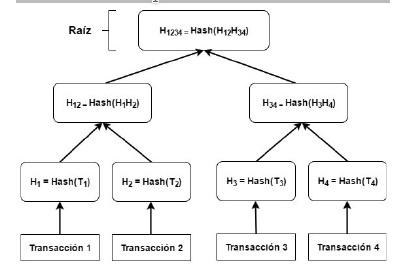
\includegraphics[scale=.75]{assets/images/arbol-hash.png}
    \caption{Arbol hash de Merkle}
\end{figure}

El árbol hash de Merkle permite almacenar la información de varias partes de manera independiente en una estructura de tipo arbol. Este arbol esta compuesto por el hash de la información en cada hoja del arbol. Los nodos de cada nivel superior se generan en base al hash de los valores del nivel inferior, se concatenan y de ese resultado se aplica una función hash. Este proceso se repite hasta llegar al nodo raíz.

La ventaja de usar este tipo de estructura en forma de árbol es que si necesitamos realizar alguna consulta, empezamos por nos nodos hoja sin la necesidad de tener toda la información generada hasta ese momento. En caso de necesitar mas información solo sera necesario subir un nivel en el arbol.

Este modelo nos ayuda a validar el contenido que hay que proporcionar a los nodos adyacentes en cada nivel y el nodo raíz. Para realizar esta validación se calcula el valor del nodo raíz a partir de los nodos adyacentes que se nos proporciona para después poder comprobar con el nodo raíz original.

Cada bloque de blockchain en la bitcoin tiene la siguiente información:

\begin{itemize}
    \item El valor hash del bloque previo.
    \item Marca de tiempo.
    \item Valor del nonce.
    \item Valor de la raíz del arbol de Merkle.
    \item Información.
\end{itemize}

\begin{figure}[htpb]
    \centering
    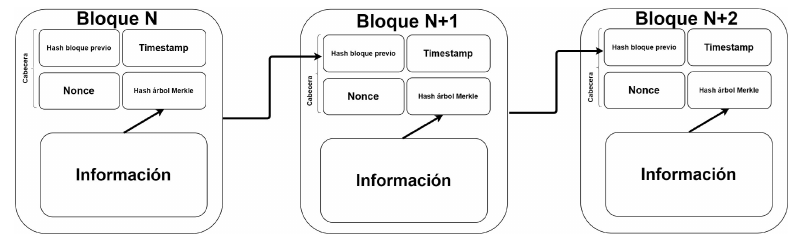
\includegraphics[scale=.4]{assets/images/bloques.png}
    \caption{Estructura de los bloques de bitcoin.}
\end{figure}

En el caso de las bitcoin la ``Información'' son los datos de las transacciones realizadas con la cripto-moneda.

\subsection{Propiedades}

Una blockchain sumamente robusta debe cumplir con las siguientes propiedades:

Disponibilidad, Una transacción exitosa acabe \\ siendo añadida a la blockchain evitando un DOS (Deny of Service) por parte de nodos corruptios.

Persistencia, Cuando un nodo da una transacción como estable, el resto de nodos, si son honestos, validarán ésta como estable haciéndola inmutable.

Para cumplir con la disponibilidad, algunas blockchain tambien implementan una red P2P (peer-to-peer) que es una red de nodos interconectados que interaccionan como pares. Esta red de igual forma es descentralizada, lo que significa que cualquier usuario que desee pueda contribuir.

Otros sistemas de blockchain en cambio utilizan un método de whitelist donde solo pueden participar los nodos que estan en esa lista. Los nodos que participen en esta red peer-to-peer disponen de una copia de la cadena de bloques. Gracias a esto es que se proporciona de una gran disponibilidad y robustez. La información que es procesada por esta red se pueden distiguir por tener varios estados como los que son:

\begin{itemize}
    \item Información candidata a ser añadida.
    \item Información confirmada.
    \item Información estable.
\end{itemize}

Hay tres caracteristicas esenciales de las blockchain y son las siguientes:

\subsection{Transparencia}

Se parte desde el punto de que todos los usuarios que forman la red de blockchain tienen acceso a la información de las transacciones. Existen algunas redes en las que los usuarios que no forman parte de la red pueden consultar dicha información, ese es el caso de las redes de bitcoin y Ethereum, además de que como es un protocolo de código abierto, cualquier persona es libre de acceder y ver como funciona este protocolo.

\subsection{Irrevocabilidad}

Una vez que los datos son validados por los nodos de la red y agregados a esta misma, es imposible que esta sea eliminada de allí. Debido a que el cambio hecho inmediatamente es distribuido a todos los nodos que conforman la red.

\subsection{Inmutabilidad}

Debido a que los bloques de información son encadenados continuamente uno detras de otro, esto se vuelve inmutable, es decir, que si un nodo decide realizar alguna modificación de la información que se encuentra en estos bloques, provocara que este cambio sea fácilmente comprobable por los demás nodos participantes de la red de blockchain y estos no aceptaran el cambio hecho debido a que el contenido no es verídico.

\section{Tipos de blockchain}

Principalmente hay 3 que surgen con la introducción de la tecnología blockchain al mundo.

\begin{figure}[htbp]
    \centering
    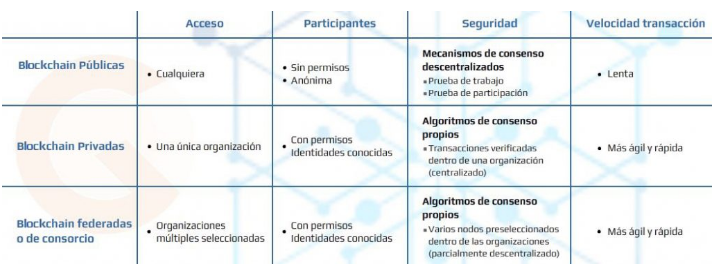
\includegraphics[scale=.4]{assets/images/tipos.png}
    \caption{Tipos de blockchain.}
\end{figure}

\subsection{Públicas}

La gran diferencia entre las blockchains públicas y privadas está relacionada con quien tiene acceso a participar en la red, ejecutando el protocolo de consenso y manteniendo la cadena de bloques.

Una red de blockchain pública es completamente abierta y cualquiera puede unirse y participar en la red. La red típicamente tiene un mecanismo de incentivación basada en la teoría de juegos que fomenta que más participantes se unan a la red. Bitcoin sigue siendo a día de hoy, la blockchain pública más grande en producción.

Una de las cuestionas que viene a nuestra mente es cómo son tomadas las decisiones en blockchains públicas. La respuesta es que como ya se ha mencionado, la toma de decisiones sucede con varios mecanismos de consenso descentralizados como Proof of Work (PoW) y Proof of Stake (PoS), etc. En entradas posteriores explicaremos en detalle cómo funcionan cada uno de ellos.

\begin{itemize}
    \item Cualquiera puede descargarse el código y empezar a correr un nodo público en sus dispositivos locales, validando transacciones en la red, de este modo participando en el proceso de consenso, el proceso para determinar que bloques son añadidos a la cadena y su estado actual.
    \item Cualquiera en el mundo puede enviar transacciones a través de la red y esperar que sean incluido en la blockchain si son válidas.
    \item Cualquiera puede real las transacciones en el explorados de transacciones públicas. Las transacciones son transparentes, pero anónimas/pseudoanónimas.
\end{itemize}

\subsection{Privadas}

Una red blockchain privada requiere una invitación que debe ser validada o bien, por el creador de la red o bien, por un grupo de reglas puestas en marcha cuando el creador creó la red.

Las compañías que abren una blockchain privada, normalmente lo hacen con una red con permisos con el fin de poner restricciones en quién puede participar en la red y realizar transacciones. El mecanismo de control de acceso puede variar; pueden ser los participantes quienes decidan futuros entrantes o puede ser una autoridad reguladora quien otorgue las licencias para participar. Una vez una entidad se ha unido a la red, jugará un rol en mantener la blockchain.



\subsection{Jurídicas o de consorcio}

Este tipo de blockchain intenta eliminar la completa autonomía de una sola entidad sobre una blockchain.

Básicamente, en este tipo de redes hay un grupo de compañías o individuales representados que se juntan para tomar mejores decisiones para toda la red. Estos grupos son llamados consorcios o federaciones.

Al contrario que en las blockchain públicas, ellos no permiten a ninguna persona con acceso a internet participar en el proceso de verificar transacciones. Las blockchain federadas son más rápidas (más escalabilidad) y proveen de mas privacidad en las transacciones.

Las blockchains de consorcio son utilizadas en el sector bancario y el sector energético.

El proceso de consenso es controlado por un grupo de nodos preseleccionados. Por ejemplo, uno se puede imaginar un grupo de 15 instituciones financieras, en la que cada una opera un nodo y de los cuales, 10 deben firmar cada bloque para que el bloque sea válido.

El derecho a leer la blockchain puede ser publica o restringida a los participantes.

\section{Tecnologías}

\subsection{Blockchain como una base de datos normal}

Las bases de datos tradicionales en línea usualmente usan una arquitectura de red cliente-servidor. Esto significa que los usuarios con derechos de acceso pueden cambiar las entradas almacenadas en la base de datos, pero el control general permanece con los administradores. Cuando se trata de una base de datos Blockchain, cada usuario está a cargo de mantener, calcular y actualizar cada nueva entrada. Cada nodo debe trabajar en conjunto para asegurarse de que llegan a las mismas conclusiones.

La arquitectura Blockchain también significa que cada nodo debe trabajar de forma independiente y comparar los resultados de su trabajo con el resto de la red. Por lo tanto, llegar a un consenso puede consumir mucho tiempo. Debido a esto, las redes Blockchain se consideran muy lentas en comparación con la tecnología tradicional de transacciones digitales.

Sin embargo, hay experimentos de producción de bases de datos con tecnología Blockchain, con BigchainDB como la primera compañía importante en el campo. Los creadores tomaron una base de datos distribuida de clase empresarial y construyeron su tecnología además de agregar los tres atributos clave de Blockchain: descentralización, inmutabilidad y la capacidad de registrar y transferir activos. Queda por determinar si lo que han creado es útil.

\subsection{ICOs (Initial Coin Offering)}

Junto con smart-contracts, se pueden intercambiar tokens por criptomoneda de acuerdo con la lógica implementada en el smart-contract. Se trata de un mecanismo utilizado cada vez más a menudo por empresas, sobre todo las conocidas como startup, para conseguir financiación para iniciar nuevos proyectos. A cambio de la criptomoneda recaudada, los emisores se comprometen a proporcionar algún tipo de valor, en muchos casos una nueva criptomoneda, si el proyecto es un éxito. \cite{blockchain4}

Lo que aportan blockchain y smart-contracts en este caso es una plataforma donde crear contratos para la recaudación de dinero y financiar proyectos de forma rápida. Al implementarse en un blockchain público y de criptomoneda, el conjunto de inversores potenciales no se restringe a un ámbito geográfico concreto. Los trámites administrativos también quedan simplificados respecto a opciones de tipo crowdfunding o empresas de capital riesgo. Como ejemplo del potencial de este mecanismo, existen casos como Filecoin o Tezos que han recaudado más de 200 millones de dólares mediante esta técnica.

\subsection{Registros públicos}

El registro de la propiedad o el catastro se está implementando en diferentes países. Los principales interesados son aquellos países donde, o bien el registro de la propiedad no existe, o bien no es confiable por ser incompleto o porque la elevada corrupción de la administración pública hace que la información no siempre sea veraz.

Diferentes países como Suecia, Grecia, Honduras o Ghana están trabajando en este tipo de soluciones. En unos casos, como el sueco, se están utilizando blockchains permissioned mientras que otros países, como Ghana u Honduras, apuestan por el registro de la información encriptada en blockchain públicos como openledger o bitcoin.

En este caso, blockchain aporta un mecanismo de registro inmutable, auditable e imposible de falsificar. En el caso de Ghana, se parte de una situación donde el registro no existe o, en el mejor de los casos, la confianza en el mismo es nula. El uso de blockchain permite eliminar los riesgos de manipulación por parte de un sistema que es, a menudo, percibido como corrupto.

\section{Aplicaciones}

Este tipo de tecnología podria ser usada en cualquier actividad que cumpla con las siguientes condiciones:

\begin{itemize}
    \item Requieran almacenar datos.
    \item El acceso a estos datos sea compartido entre diferentes partes.
    \item Estas partes no se conozcan o no tengan confianza entre ellas.
\end{itemize}

\subsection{Criptomonedas}

Las criptomonedas o monedas virtuales es un tipo de dinero dígital y no regulado, que es emitido y controlado por quienes lo desarrollan, ademas de que es usado por personas de la misma asociación. Estas monedas virtuales no estan asociadas a ninguna moneda establecida legalmente, no son emitidas por entidades publicas.

Estas criptomonedas son creadas, distribuidas e intercambiadas bajo la tecnología de blockchain. Hoy en día existen miles de criptomonedas, las más conocidas son:

\begin{itemize}
    \item Bitcoin,  diseñada para funcionar como medio de pago entre aquellos que deciden voluntariamente aceptarlo como tal.
    \item Ethereum, permite realizar transacciones más sofisticadas que el mero pago, aladmitir que operen sobre su estructura ciertos smart contracts.
\end{itemize}

\subsection{Smart contracts}

Los smart contracts o contratos inteligentes, comúnmente
conocidos como contratos autoejecutables, no es mas que un programa
autoejecutable que facilita, asegura, hace cumplir y ejecuta acuerdos registrados entre dos o más partes. Estos acuerdos se dan a través de página web accesible por las partes interesadas y esta constituida por la interfaz de usuario externa y los smart contracts.

Los smart contracts consiguen acuerdos sencillos sin ne-\\cesidad de que estos dependan de terceras personas. Es prácticamente un conjunto de reglas o acuerdos por parte de los interesados para poder llevar a cabo el contrado.

Las aplicaciones de los smart contracts se han apuntado en múltiples sectores. En el sector de los seguros, por ejemplo, se ha descrito su utilización para el pago automático de indemnizaciones una vez constatado el acaecimiento de ciertos tipos de siniestros.

\subsection{Sistema de distribución de firmware}

El internet de las cosas ha estado en incremento estos últimos años, esto significa que cada vez mas dispositivos estan conectados a la red y podemos interactuar con ellos de una manera sencilla. Esto es una gran ventaja pero implica que se debe mejorar y arreglar las posibles brechas de seguridad que puedan existir.

La administración de estos dispositivos es de cierta manera difícil ya que no todos los fabricantes de estos dan soporte, ni mantienen actualizado el firmware de estos lo que conlleva a que haya vulnerabilidades frecuentemente en este tipo de dispositivos.

El blockchain es un candidato perfecto para solucionar este problema debido a que su arquitectura esta basada en una red distribuida, ademas de que es robusto, transparente y fiable. Un dispositivo conectado a esta red de blockchain podria pedir una actualización del firmware y posterior a esto gracias al blockchain poder comprobar si el firmware ha sido alterado de alguna forma. Esto asegura que las actualizaciones del firmware no hayan sido modificadas por terceros y arreglaria de alguna forma esa brecha de seguridad.

\section{Relación con las tablas hash}

La información guardad dentro de los bloques de blockchain utilizan una función hash criptográfica que permite cifrar los datos y proteger estos mediante el uso de claves. Al aplicarla, se toma un mensaje de cualquier tamaño, se cifra, y se consigue a cambio una cadena alfanumérica única de longitud fija (llamada digest o simplemente hash), sin importar el tamaño del mensaje original. Funciona para verificar que, en efecto, se trata de ese mensaje (o transacción) en particular y que no fue modificado antes de su entrega. Si una sola parte, aunque sea un solo punto del mensaje original cambia, el hash (digest) también lo hace de forma radical.

\begin{figure}[htbp]
    \centering
    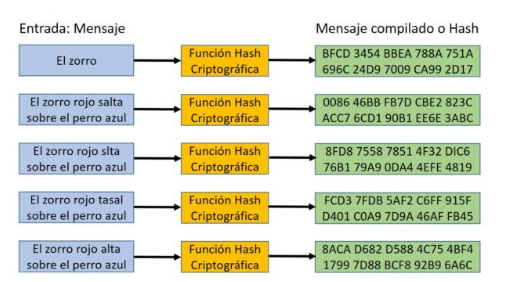
\includegraphics[scale=.6]{assets/images/hash.png}
    \caption{Encriptación por hash}
\end{figure}

\subsection{Propiedades de una funcion hash}

Las funciones hash para que puedan ser seguron deben cumplir con las siguientes catacterísticas:

\begin{itemize}
    \item Computacionalmente eficiente, ser capaces de lograr encriptar la información en el menor tiempo posible sin desperdiciar recursos.
    \item Determinista, Esto implica que el mismo mensaje (entrada) debe producir siempre el mismo digest (salida) cada vez que sea utilizado o consultado.
    \item Resistente a preimagen, significa que los datos de entrada no deben ser revelados en la salida.
    \item Resistente a colisión, cada entrada tiene una unica salida, no puede haber diferentes entradas con la misma salida.
\end{itemize}

\bibliographystyle{plainnat}
\bibliography{biblo.bib}

\end{document}
